\documentclass[border=4pt]{standalone}
\usepackage{amsmath,amssymb}
\usepackage{tikz}
\usetikzlibrary{arrows.meta,shadows}
\begin{document}
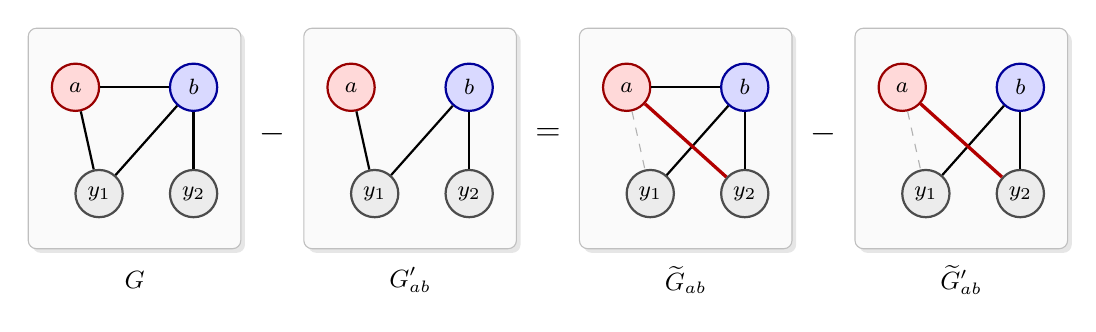
\begin{tikzpicture}[
  vx/.style={circle,draw=#1!60!black,fill=#1!15,thick,minimum size=6mm,font=\footnotesize,inner sep=0pt},
  e/.style={thick},
  ne/.style={very thick,red!70!black},
  panel/.style={draw=gray!50,fill=gray!4,rounded corners=3pt,
                drop shadow={opacity=0.2,shadow xshift=1.5pt,shadow yshift=-1.5pt}}]
  \newcommand{\fourpanel}[5]{% #1 x-shift, #2 ab edge, #3 a-y edges, #4 label, #5 other
    \begin{scope}[xshift=#1cm]
      \draw[panel] (-1.35,-1.45) rectangle (1.35,1.35);
      \node[vx=red]  (a)  at (-0.75,0.6) {$a$};
      \node[vx=blue] (b)  at (0.75,0.6)  {$b$};
      \node[vx=gray] (y1) at (-0.45,-0.75) {$y_1$};
      \node[vx=gray] (y2) at (0.75,-0.75)  {$y_2$};
      \draw[e] (b) -- (y1); \draw[e] (b) -- (y2);
      #2 #3 #5
      \node[font=\small] at (0,-1.85) {#4};
    \end{scope}}
  \fourpanel{0}{\draw[e] (a) -- (b);}{}{$G$}{\draw[e] (a) -- (y1);}
  \fourpanel{3.5}{}{}{$G'_{ab}$}{\draw[e] (a) -- (y1);}
  \fourpanel{7.0}{\draw[e] (a) -- (b);}{\draw[ne] (a) -- (y2);}{$\widetilde G_{ab}$}{\draw[dashed,gray!60] (a) -- (y1);}
  \fourpanel{10.5}{}{\draw[ne] (a) -- (y2);}{$\widetilde G'_{ab}$}{\draw[dashed,gray!60] (a) -- (y1);}
  \node[font=\large] at (1.75,0) {$-$};
  \node[font=\large] at (5.25,0) {$=$};
  \node[font=\large] at (8.75,0) {$-$};
\end{tikzpicture}
\end{document}
